%!TEX root = ../main.tex

\chapter{Impianti}
\label{chp:impianti}
Nel capitolo precedente sono state elencate e brevemente introdotte le varie fonti energetiche che abbiamo a disposizione. Sarà obbiettivo di questo capitolo elencare ed illustrare il funzionamento degli impianti utilizzabili per convertire le varie fonti energetiche in energia elettrica la quale sarà poi immessa nella rete elettrica.\\
\section{Impianto fotovoltaico}
Un impianto fotovoltaico è un impianto elettrico formato da più moduli fotovoltaici i quali, sfruttando l'energia solare, producono energia elettrica mediante il così detto l'effetto fotovoltaico.\\
All'interno di un impianto fotovoltaico possiamo identificare alcuni elementi chiave e fondamentali come:
\begin{itemize}
    \item Cavi, diodi e magnetotermici
    \item Inverter
\end{itemize}
I primi sono fondamentali per la connessione e la sicurezza dell'impianto mentre i secondi sono necessari per la conversione DC-AC per poi poter immettere in rete l'energia elettrica che si produce.\\
Per illustrare il funzionamento di un impianto è importante prima capire il funzionamento dell'effetto fotovoltaico.\\
\subsection{Effetto fotovoltaico}
Durante lo studio delle onde elettromagnetiche si notò come una radiazione elettromagnetica che investe un materiale possa, in certe condizioni, cedere energia agli elettroni più esterni degli atomi del materiale stesso. Se l'energia risulta sufficiente l'elettrone è libero di staccarsi dall'atomo di origine ed allontanarsi.\\
Questo fenomeno però non può essere sfruttato in tutti i materiali. Negli isolanti, per esempio, il gap tra la banda di condizione e la banda di valenza, chiamato band gap, è troppo elevato per poter essere eguagliato dall'energia del fotone incidente. Per i materiali conduttori, invece, vi è una continua creazione e distruzione di coppie elettrone-lacune e l'energia necessaria per la creazione di esse viene fornita direttamente dalla variazione di temperatura.\\
Al contrario, quando un fascio luminoso investe un semiconduttore si verifica il passaggio in banda di conduzione di un certo numero di elettroni al quale corrisponde un uguale numero di lacune che passa in banda di valenza.\\
Per generare un flusso di elettroni è necessario creare un campo elettrico all'interno della cella, per tale scopo si sfrutta il drogaggio. Il drogaggio consiste nell'inserire atomi diversi dal silicio all'interno di alcune zone del semiconduttore per ottenere due zone: la prima con eccesso di lacune(zona p) la seconda con eccesso di elettroni(zona n).\\
\begin{figure}[H]
    \centering
    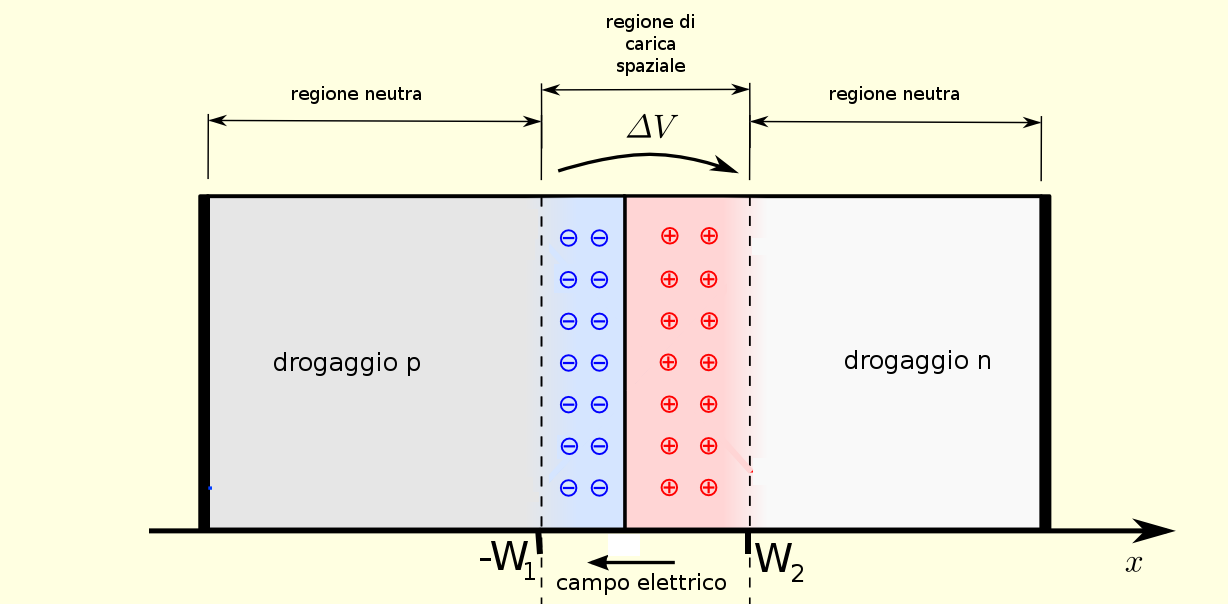
\includegraphics[height=0.5\textwidth]{res/cap 3/drogaggio}
    \caption{Rappresentazione di semiconduttore con drogaggio p-n}
\end{figure}\noindent
Si formano quindi due zone, la prima con una prevalenza di elettroni liberi e la seconda con lacune le quali provocano una carenza di elettroni andandosi a creare un campo elettrico che si estende a cavallo della regione di svuotamento.
Grazie al fenomeno illustrato in precedenza se si illumina la giunzione dalla parte n vengono a crearsi delle copie elettrone-lacune in entrambe le zone, il campo elettrico presente a causa del drogaggio fa si che gli elettroni in eccesso si dividano e li spinge in direzioni opposte. Una volta oltrepassata la regione di svuotamento non possono quindi più tornare indietro a causa della presenza del campo elettrico.\\
Procedendo quindi con una connessione esterna si otterrà un circuito chiuso nel quale il flusso di elettroni parte dallo strato n,a potenziale maggiore, per dirigersi nello strato p, a potenziale minore fintanto che la cella rimanere esposta ai raggi solari.\\
\subsection{Cella solare}
Una cella solare è un dispositivo elettrico a stato solido il quale tramite l'effetto fotovoltaico permette di convertire l'energia trasportata dalla luce solare in elettricità tramite l'effetto illustrato nella sezione precedente.\\
La maggior parte delle celle fotovoltaiche prodotte, se esposte al sole, producono una tensione di circa 0.6V, è quindi necessario metterle in serie per ottenere tensioni più alte.
Collegando le celle in serie però non si ha il controllo sulle singole celle in quanto la stessa corrente attraversa tutte le celle, quelle poste in ombra quindi finiscono per fare da strozzatura per tutto il sistema andando a scaldarsi e potenzialmente a danneggiarsi.\\
E' quindi visibile l'importanza di posizionare correttamente i pannelli fotovoltaici in modo che vi siano delle zone d'ombra e per meno periodi possibili.\\
\subsection{Pannello fotovoltaico}
\paragraph{Struttura}\mbox{}\\
Un pannello fotovoltaico è formato da un'insieme di celle opportunamente collegate tramite una griglia metallica che è presente sulla superficie del modulo in modo da formare sia collegamenti in serie che in parallelo. Una volta collegate le celle si procede con l'assemblaggio del modulo ponendo sopra la superficie posteriore, realizzata con un materiale isolante con scarsa dilatazione termica, uno strato di acetato di vinile(EVA), si pone quindi lo strato di celle solare opportunamente collegate per poi porre un'ulteriore strato di EVA ed il vetro temperato a protezione dell'intero modulo.\\
\begin{figure}[H]
    \centering
    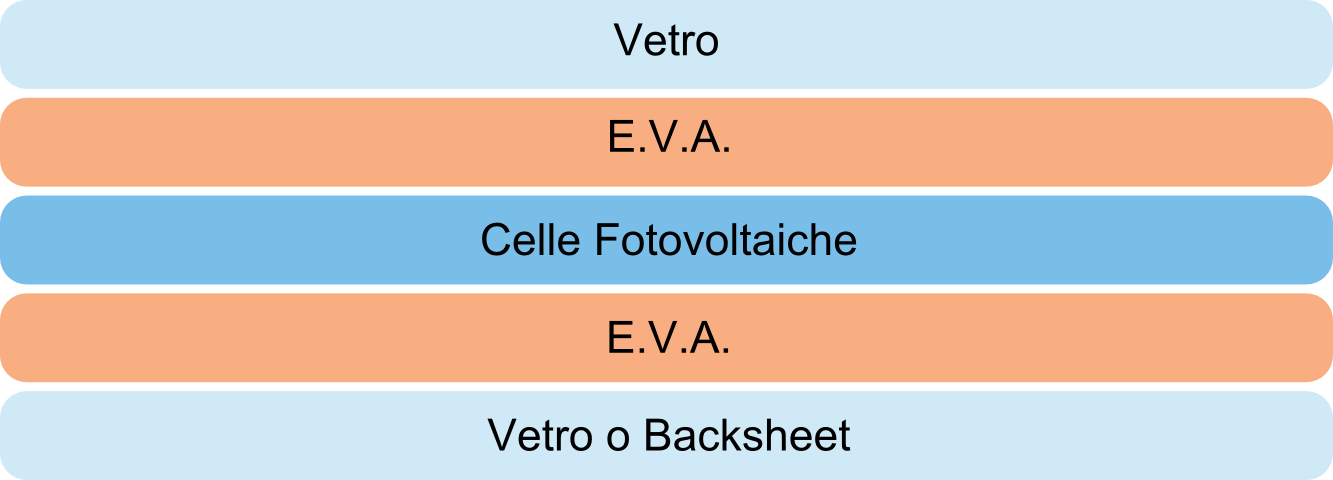
\includegraphics[height=0.3\textwidth]{res/cap 3/composizione modulo}
    \caption{Schema di composizione di un modulo fotovoltaico}
\end{figure}\noindent
Una volta assemblato si procede con un processo di pressofusione atto a trasformare l'EVA in un collante inerte, si collega la griglia ad una morsettiera che viene posta sul retro e si chiude il modulo in un frame di alluminio che faciliterà l'installazione e l'orientamento.
\paragraph{Tecnologie realizzative}\mbox{}\\
Dei molti semiconduttori utilizzabili per la produzione dei moduli fotovoltaici il più comunemente usato è il silicio, esso si ottiene in wafer che successivamente vengono uniti tra loro a formare un modulo.\\
Esistono diverse tipologie costruttive delle celle, tra le più comuni troviamo:
\begin{description}[labelindent=5mm]
    \item[$\cdot$ Silicio monocristallino:] ogni cella è realizzata a partire da un wafer formato da un monocristallo opportunamente drogato. Sono tendenzialmente costose in quanto risulta difficile formare ampie superfici senza sprecare materiale o spazio, però permettono di raggiungere un'efficienza dell'ordine del 18-21\%.
    \item[$\cdot$ Silicio policristallino:] in questo caso la cella è formata da un policristallo, quindi non strutturalmente omogeneo ma organizzato in grani localmente ordinati. Il costo in questo caso data la peggior qualità del silicio usato risulta più basso a favora di una maggior facilità di taglio e lavorazione. L'efficienza raggiungibile con questa tipologia di silicio però è più bassa del caso precedente e si attesta nell'ordine del 15-17\%. 
    \item[$\cdot$ Silicio amorfo:] questa tipologia di celle hanno un'efficienza più bassa ($\sim8\%$) ma risultano molto più economici da produrre rispetto ad i precedenti. Il silicio amorfo ha un bandgap più ambio dei precedenti(circa un 55\% in più) il che favorisce l'assorbimento della parte visibile dello spettro solare ma risulta meno efficiente nell'elaborare la parte infrarossa.
\end{description}
\paragraph{Prestazioni ed efficienza}\mbox{}\\
Le prestazioni offerte dal singolo modulo dipendono da diversi fattori, in prima fase, si può calcolare, in modo approssimato, la potenza che un pannello è in grado di esprimere con la seguente formula:
\begin{center}
    \large{$P = \eta I_0 S \sin(\alpha)  $}
\end{center}
Dove con $I_0$ si considera l'irradianza perpendicolare alla superficie, con S la superficie del modulo, mentre $\alpha$ è l'angolo che il modulo ha con il sole, $\eta$ invece è un fattore di rendimento.\\
In conclusione possiamo osservare come i parametri fisici che influenzano la produzione di un pannello solare possano essere sintetizzati in:
\begin{itemize}
    \item Irraggiamento a cui il pannello è esposto
    \item Angolo con la quale in modulo è orientato
    \item Qualità produttiva del modulo
    \item Tipologia di silicio usato
\end{itemize}
Si nota anche qui l'importanza di collocare il pannello in una regione che abbiamo una buona copertura da parte del sole ed in una superficie correttamente orientata.\\
Nel caso di installazioni su tetti questi due parametri rendono o meno un determinato tetto idoneo all'installazione, nel caso si installino in campi fotovoltaici invece l'angolo di installazione viene scelto in fase costruttiva quindi ideale per il luogo in cui è collocato.\\
Come visto in precedenza l'angolo con cui la luce solare colpisce la terra dipende sia dal luogo geografico che dal periodo dell'anno preso in esame, vi sarà quindi un'efficienza diversa da periodo data dall'inclinazione del modulo oltre che dalle condizioni climatiche.\\
Il singolo modulo in condizioni normali lavora in un range di tensione a vuoto($V_{OC}$) tra 40 ed i 50 Volt ed una corrente di cortocircuito($I_{sc}$) tra i 9 ed i 12 Ampere.\\
Un altro fattore importante che influenza negativamente il rendimento di un pannello fotovoltaico è la temperatura, infatti la temperatura della giunzione p-n va ad influenzare sia ($V_{OC}$) che ($I_{sc}$) andando quindi ad alterare anche la potenza massima($P_{Max}$) che il modulo è in grado di offrire.\\
Per quantificare l'impatto della temperatura sul pannello ogni produttore fornisce tre valori tre espressi in $\frac{\%}{^\circ C}$:
\begin{enumerate}
    \item Coefficiente di temperatura di ($P_{Max}$)
    \item Coefficiente di temperatura di ($V_{OC}$)
    \item Coefficiente di temperatura di ($I_{sc}$)
\end{enumerate}
\newpage
\section{Impianto eolico}
Un impianto eolico è un sistema che converte l'energia del vento in energia elettrica.
Gli elementi fondamentali che lo compongono sono:
\begin{description}[labelindent=5mm]
    \item[$\bullet$ Pale eoliche]: sono le parti rotanti che catturano l'energia del vento, deve essere possibile variarne l'angolo di calettamento per ottimizzarne il funzionamento.
    \item[$\bullet$ Moltiplicatore di giri]: consente di prendere in input un certo numero di giri ad una determinata coppia e dare in output un numero superiore di giri ad una coppia più bassa.
    \item[$\bullet$ Generatore eolico]: è un dispositivo che converte l'energia meccanica generata dalla rotazione delle pale in energia elettrica.
    \item[$\bullet$ Torre eolica]: sostiene le pale ed il generatore permettendone l'installazione ad un'altezza adeguata per catturare il vento in maniera adeguata.
    \item[$\bullet$ Elettronica di controllo] controlla il funzionamento complessivo dell'impianto con lo scopo di mantenere alte performance e standard di sicurezza elevati.
\item \end{description}
A questi elementi principali che compongono un impianto eolico si possono aggiungere, a seconda delle dimensioni e delle esigenze, altri componenti come inverter, sistemi di raffreddamento.
Saranno ora brevemente illustrati i vari componenti e ne sarà spiegato in modo sintetico il funzionamento e principi che li guidano.
Una prima suddivisione va fatta in base alle forma, infatti esistono fondamentalmente due tipi di turbine:
\begin{itemize}
    \item \textbf{HAWT} (Horizontal Axis Wind Turbines)
    \item \textbf{VAWT} (Vertical Axis Wind Turbines)
\end{itemize}
Le prime possono essere configurate sia con rotore sopravvento che sottovento, nel primo caso si ha il vantaggio di non avere interferenza di alcun tipo da parte della torre mentre nel secondo caso la macchina è in grado di orientarsi in automatico.
Nel caso di turbine VAMT,invece, vi è la caratteristica di essere immuni alla direzione del vento ma tendenzialmente avere una resa rispetto allo spazio occupato inferiore rispetto al caso precedente.
\subsection{Caratteristiche e casi d'uso HAWT e VAWT}
\paragraph{HAWT}\mbox{}\\
Le caratteristiche principali di una turbina eolica a elica orizzontale (HAWT) sono le seguenti:
\begin{description}[labelindent=5mm]
    \item[$\bullet$ Alta efficienza]: Le turbine HAWT sono progettate per catturare l'energia del vento in modo efficiente, con rendimenti più elevati rispetto alle turbine VAWT.
    \item[$\bullet$ Adatte ai venti forti]: Le turbine HAWT sono particolarmente adatte ai venti forti, poiché la loro progettazione a elica orizzontale le rende in grado di catturare l'energia del vento in modo più efficiente.
    \item[$\bullet$ Dimensioni maggiori]: Le turbine HAWT sono generalmente più grandi delle turbine VAWT, il che le rende adatte per l'installazione in aree con spazi più ampi.
    \item[$\bullet$ Funzionamento più rumoroso]: Le turbine HAWT possono essere più rumorose delle turbine VAWT, poiché l'elica che gira rapidamente è più vicina alla superficie terrestre.
\end{description}
Date le caratteristiche peculiari di questa tipologia di turbine alcuni casi d'applicazione possono essere:
\begin{description}[labelindent=5mm]
    \item[$\bullet$ Impianti di grandi dimensioni]: Le turbine HAWT sono adatte per la costruzione di impianti di grandi dimensioni, infatti possono produrre grandi quantità di energia elettrica.
    \item[$\bullet$ Parchi eolici]: Le turbine HAWT sono spesso utilizzate per la costruzione di parchi eolici, dove vengono installate molte turbine per produrre energia elettrica a livello commerciale.
    \item[$\bullet$ Installazioni offshore]: Le turbine HAWT possono essere installate in mare per sfruttare i venti più forti che soffiano al largo della costa.
    \item[$\bullet$ Alimentazione elettrica per grandi comunità]: Le turbine HAWT possono essere utilizzate per fornire energia elettrica a grandi comunità, come città e fabbriche.
\end{description}
Le turbine di tipologia HAWT sono l'unica opzione percorribile quando lo scopo dell'installazione è generare grandi quantità di energia in presenza di venti di intensità sostenuta.
Tuttavia essendo particolarmente rumorose e visivamente impattanti la loro installazione è spesso effettuata offshore o a distanza dalle comunità.
\begin{figure}[H]
    \centering
    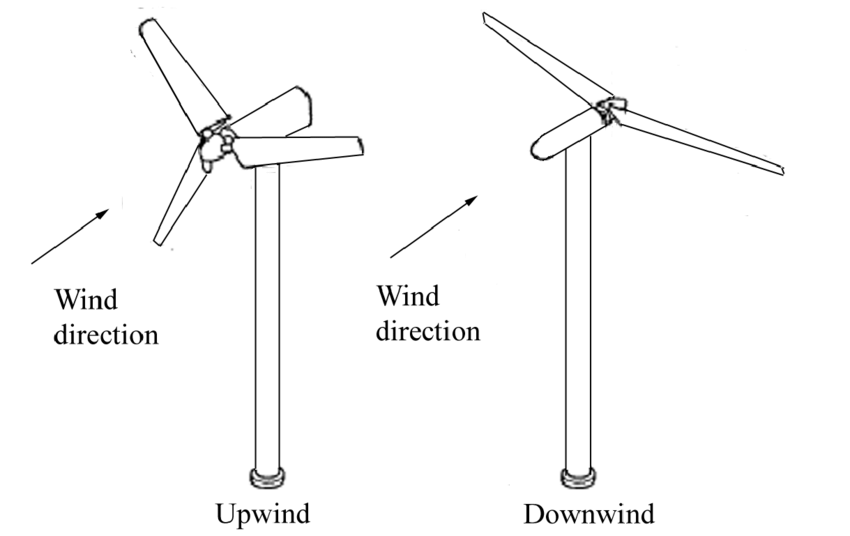
\includegraphics[height=0.3\textwidth]{res/cap 3/HAWT}
    \caption{Esempio di turbina HAWT sopravvento e sottovento}
\end{figure}\noindent
\paragraph{VAWT}\mbox{}\\
Le caratteristiche principali di una turbina eolica ad elica verticale (VAWT) sono le seguenti:
\begin{description}[labelindent=5mm]
    \item[$\bullet$ Design compatto]: Le pale sono disposte verticalmente, il che le rende più compatte e adatte per l'installazione in aree limitate.
    \item[$\bullet$ Funzionamento silenzioso]: Sono progettate per funzionare in modo più silenzioso rispetto alle pale HAWT (a elica orizzontale), poiché non vi è un'elica che gira rapidamente nella vicinanza della superficie terrestre generando quindi meno rumore.
    \item[$\bullet$ Minor influenza dal vento irregolare]: Sono meno influenzate dal vento irregolare rispetto alle pale HAWT, poiché il loro design a elica verticale le rende più stabili e meno sensibili alle perturbazioni del vento.
    \item[$\bullet$ Adatte per venti deboli]: Sono particolarmente adatte per i venti deboli, poiché possono catturare energia dai venti deboli che soffiano in direzioni diverse rispetto alle pale HAWT che necessitano di venti di direzione costante e di intensità più sostenuta.
\end{description}
Date le caratteristiche appena descritte i casi specifici di applicazione che si possono identificare sono i seguenti:
\begin{description}[labelindent=5mm]
    \item[$\bullet$ Piccole comunità rurali]: Le turbine VAWT possono essere utilizzate per fornire energia elettrica a piccole comunità rurali che altrimenti non sarebbero in grado di accedere ai servizi di energia elettrica.
    \item[$\bullet$ Sistemi di energia solare ibridi]: Le turbine VAWT possono essere utilizzate insieme a sistemi di energia solare per fornire un'alimentazione elettrica affidabile durante tutto l'anno.
    \item[$\bullet$ Edifici residenziali e commerciali]: Le turbine VAWT possono essere utilizzate per fornire energia elettrica a edifici residenziali e commerciali, riducendo la loro dipendenza dalla rete elettrica nazionale.
    \item[$\bullet$ Sistemi di energia marini]: Le turbine VAWT possono essere utilizzate per fornire energia elettrica a sistemi di energia marini, come piattaforme petrolifere e rig.
\end{description}
Le turbine di tipologia VAWT sono un'opzione valida per fornire energia elettrica in tutte quelle situazioni in cui sono necessarie turbine compatte, silenziose e adatte ai venti deboli.
Tuttavia, il loro rendimento è generalmente inferiore rispetto alle pale HAWT, quindi potrebbero non essere la scelta migliore per grandi campi eolici.
\begin{figure}[H]
    \centering
    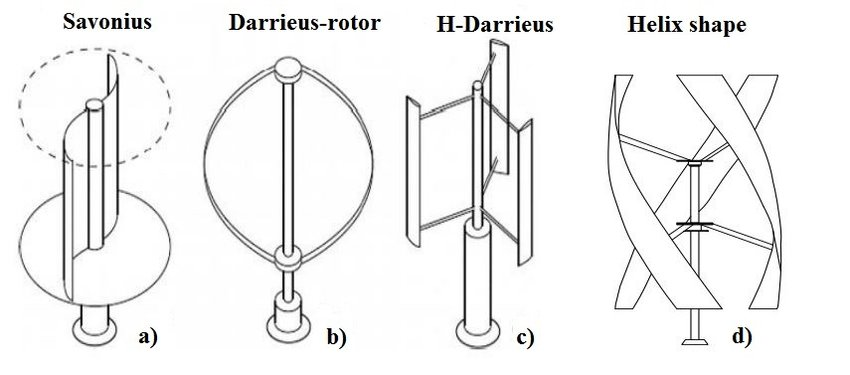
\includegraphics[height=0.3\textwidth]{res/cap 3/VAWT}
    \caption{Esempio di diverse tipologie di turbine VAWT}
\end{figure}\noindent
\subsection{Prestazioni ed efficienza}
Per descrivere questo capitolo è importante parlare e specificare il limite di betz in quanto pone il limite superiore di efficienza raggiungibile da qualsiasi impianto eolico.\\
Il limite di Betz porta a descrivere il rendimento come segue è espresso come segue:\\
{\large$\eta = \frac{16}{27} \cdot (1 - (\frac{v_2}{v_1})^2)$}\\
dove:\\
{\large$\eta$} è il coefficiente di prestazione (rendimento) della turbina eolica\\
{\large$v_1$} è la velocità del vento all'ingresso della turbina\\
{\large$v_2$} è la velocità del vento all'uscita della turbina.\\
Il limite di Betz rappresenta il massimo rendimento teorico che può essere ottenuto da una turbina eolica corrisponde a un coefficiente di prestazione pari a $\frac{16}{27}$ pari a circa il 60\%.\\
Nella pratica, le turbine eoliche reali hanno rendimenti molto più bassi, solitamente compresi tra il 20\% e il 50\% a causa di fattori come la resistenza dell'aria, la turbolenza e la frizione all'interno della turbina. Tuttavia, il limite di Betz fornisce un punto di riferimento importante per la valutazione dell'efficienza delle turbine eoliche.
\paragraph{HAWT}\mbox{}\\
Le prestazioni e l'efficienza delle turbine eoliche a elica orizzontale (HAWT) sono determinate da una serie di fattori, tra cui la velocità del vento, la densità dell'aria, la geometria della turbina e la tecnologia utilizzata.
L'efficienza delle turbine HAWT può essere valutata utilizzando il coefficiente di prestazione, che rappresenta la quantità di energia catturata dalla turbina rispetto all'energia del vento disponibile.\\
In generale, come visto sopra, le turbine HAWT hanno coefficienti di prestazione compresi tra il 40\% e il 50\%.\\
La velocità del vento è un fattore critico per le prestazioni delle turbine HAWT. A velocità del vento maggiori, la turbina produce più energia elettrica. Tuttavia, se la velocità del vento supera un certo limite, la turbina può essere danneggiata o subire un arresto di sicurezza.\\
La tecnologia utilizzata nelle turbine HAWT influisce anche sulle prestazioni. Ad esempio, l'utilizzo di materiali leggeri e resistenti come la fibra di carbonio può aumentare la durata e la resistenza delle pale della turbina, migliorando le prestazioni a fronte però di un sostanzioso aumento dei costi costruttivi.\\
Inoltre, l'utilizzo di sistemi di controllo avanzati può aiutare a ottimizzare la produzione di energia elettrica in base alle condizioni del vento andando ad esempio a far variare l'angolo di attacco delle pale in modo da adattarlo alla velocità del vento presente ottimizzando i flussi.
\paragraph{VAWT}\mbox{}\\
Le turbine VAWT hanno alcune caratteristiche uniche che le rendono adatte a determinate situazioni e poco adatte per altre per questo motivo si utilizzano, non per cercare una grande efficienza, ma quando il caso specifico lo richiede.
In termini di prestazioni, le turbine VAWT hanno una efficienza inferiore rispetto alle turbine HAWT, la quale si attesta generalmente intorno al 30-40\%.
Si nota come questo range sia inferiore rispetto a quello riscontrato nelle turbine HAWT però compensato dalla possibilità di essere inserite in contesti particolari e di richiedere mediamente meno manutenzione e garantendo una maggior semplicità di installazione non dovendo ad esempio essere orientate.
\newpage
\section{Centrale a biomasse}
La tipologia di impianti che sfruttano la digestione anaerobica per produrre biogas il quale andrà ad alimentare una caldaia.\\
Concentrandoci su questa tipologia di impianti è importante descrivere le fasi che la compongono:\\
\begin{description}[labelindent=5mm]
    \item[$\bullet$ Produzione di acidi grassi]: i batteri scompongono gli zuccheri, amidi e grassi presenti nella biomassa in acidi grassi, come l'acido solfidrico e l'acido lattico.
    \item[$\bullet$ Fermentazione]: gli acidi grassi vengono ulteriormente decomposti da altri batteri anaerobici in biossido di carbonio (CO2) e metano (CH4). Questo processo è chiamato fermentazione acida o acidogenesi.
    \item[$\bullet$ Maturazione]: durante questa fase, i resti della digestione anaerobica vengono trasformati in compost stabile da batteri aerobi. Questo compost può essere utilizzato come fertilizzante per la coltivazione di piante.
\end{description}
Tali processi avvengono all'interno di un digestore dal quale si avrà come risultato il biogas ed il substrato digerito, il quale sarà ricco di sostanze come: azoto, fosforo, potassio.
La quantità di biogas che si è in grado di estrarre dipende da diversi fattori quali:
\begin{description}[labelindent=5mm]
    \item[$\bullet$ Composizione chimica della biomassa]: la quantità di biogas prodotta dipende dalla quantità e dalla qualità dei componenti presenti nella biomassa, come ad esempio zuccheri, amidi, proteine e grassi.
    \item[$\bullet$ Condizioni ambientali]: il pH cioè la temperatura ed il tempo di digestione.
    \item[$\bullet$ Tipo di batteri]: il tipo di batteri utilizzati e dalla loro capacità di decomporre la biomassa in biogas.
    \item[$\bullet$ Dimensione e tecnologia dell'impianto]: vi è una dipendenza anche dalla capacità dell'impianto e dalla tecnologia utilizzata per la digestione anaerobica(presenza di sistemi di miscelazione o di controllo di processo).
\end{description}
Il processo necessita della presenza di batteri, i quali andranno a decomporre la sostanza organica. Vi sono 3 tipi di batteri diversi che operano a diverse temperature ed hanno tempi di permanenza nel reattore diversi:\\
\begin{description}[labelindent=5mm]
    \item[$\bullet$ Batteri psicrofili]: sono batteri che si sviluppano a temperature comprese tra 5°C e 25°C. Sono adatti a processi che avvengono a temperature più basse.La loro permanenza nel sistema di digestione è di circa 10-12 settimane.
    \item[$\bullet$ Batteri mesofili]: sono batteri che si sviluppano a temperature comprese tra 25°C e 45°C. Sono adatti a processi che avvengono a temperature medie e la loro permanenza è di circa 3-8 settimane.
    \item[$\bullet$ Batteri termofili]: sono batteri che si sviluppano a temperature comprese tra 45°C e 60°C. Sono adatti a processi che avvengono a temperature elevate e la loro permanenza è di circa 2-3 settimane.
\end{description}
\vfill
\newpage
La scelta del tipo di batteri da utilizzare dipende,in generale, dalle condizioni ambientali e dal tipo di biomassa che si desidera trattare. La selezione dei batteri più adatti aumenta l'efficienza e la quantità di biogas prodotto durante la digestione anaerobica.\\
\begin{figure}[H]
    \centering
    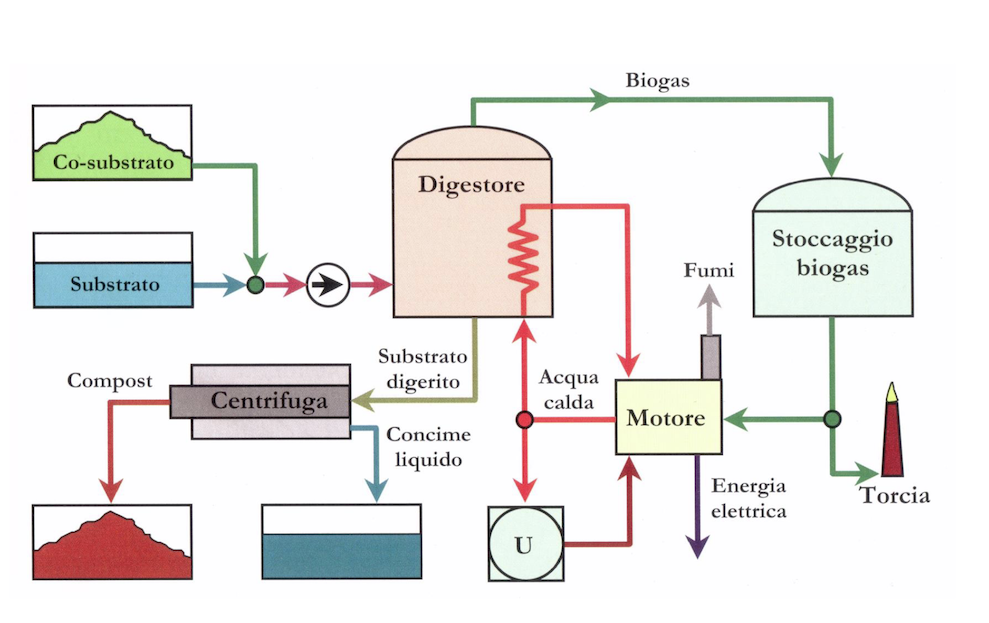
\includegraphics[height=0.5\textwidth]{res/cap 3/Biomasse}
    \caption{Esempio di uno schema di un impianto a biomasse con digestore anaerobico\cite{Materiale_didattico_prof_savino}}
\end{figure}\noindent
\section{Impianti per correnti marine}
Questa tipologia di impianti sfrutta l'energia cinetica delle correnti marine per produrre energia elettrica.\\
Vengono utilizzate turbine a elica simili a quelle utilizzate nei generatori eolici per trasformare l'energia cinetica dell'acqua in energia meccanica, che viene poi convertita in energia elettrica attraverso l'utilizzo di generatori elettrici.\\
Le turbine a elica possono essere sia collocate su una struttura galleggiante che su una fissa fissa la quale è comunque ancorata al fondale marino.
La produzione di energia è direttamente proporzionale alla velocità della corrente e alla superficie della turbina da qui l'importanza di effettuare una corretta scelta di posizionamento e dimensionamento dell'impianto, scelta che influenza poi alcune scelte costruttive e strutturali.
Esistono infatti due tipi principali di turbine ad elica utilizzate negli impianti a energia delle correnti marine: le turbine ad asse orizzontale e le turbine ad asse verticale.\\
Le turbine ad asse orizzontale, simili a quelle utilizzate nei generatori eolici, hanno le pale dell'elica montate su un asse orizzontale che ruota intorno ad un mozzo centrale.\\
Le turbine ad asse verticale, invece, hanno le pale dell'elica montate su un asse verticale che ruota intorno a un mozzo centrale.\\
\begin{figure}[H]
    \centering
    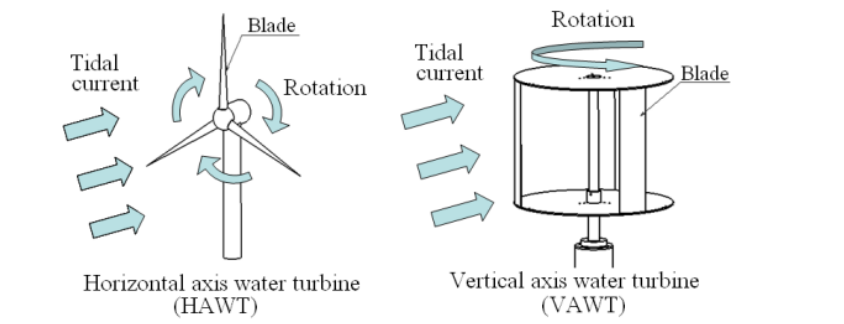
\includegraphics[height=0.4\textwidth]{res/cap 3/Ocean current turbine}
    \caption{Esempio di varie tipologie di turbine ad asse verticale\cite{Ocean_current_turbine}}
\end{figure}\noindent
La scelta della tipologia di turbina da utilizzare dipende quindi dalle condizioni dell'ambiente in cui l'impianto viene installato: le turbine ad asse orizzontale, ad esempio, sono più adatte per acque poco profonde e correnti con una direzione del flusso costante, mentre le turbine ad asse verticale sono più adatte per acque più profonde e correnti con una direzione del flusso variabile.\\
Gli impianti che sfruttano l'energia delle correnti marine presentano alcuni vantaggi rispetto ad altre tecnologie di produzione di energia rinnovabile: in particolare, le correnti marine sono costanti e prevedibili, ciò significa che la produzione di energia è più affidabile e continua rispetto ad altre fonti di energia rinnovabile.
Inoltre non interferiscono con le attività di pesca o la navigazione che possono avvenire in totale normalità a patto che l'impianto sia stato correttamente progettato e posizionato.\\
Di contro, gli impianti a energia delle correnti marine possono avere anche un impatto negativo sull'ambiente marino e sulla vita marina se la loro struttura non è costruita in modo da impedire contatti accidentali con le parti in movimento.\\
\section{Centrali mareomotrici}
Le centrali mareomotrici sono tutta quella tipologia di impianti che sfruttano l'energia mareomotrice che si ricava dallo spostamento dell'acqua causato dalle maree.\\
Si possono identificare quattro tipologia di impianti che sfruttano l'energia delle maree ma il funzionamento finale è molto simile per tutti:\\
\begin{itemize}
    \item Sollevamento di un peso
    \item Compressione dell'acqua in opportuni cassoni e movimentazione delle turbine in espansione
    \item Mobimento di ruote a pale(più usato nell'antichità che in epoca moderna)
    \item Riempimento di bacini e successivo svuotamento con passaggio(sia in ingresso che in uscita) attraverso turbine
\end{itemize}
Sarà illustrato il funzionamento degli impianti a bacino in quanto sono i maggiormente usati per sfruttare questa tipologia di fenomeno.\\
\subsection{Impianti a bacino}
In questa tipologia di impianto, l'energia delle maree viene utilizzata per riempire un bacino artificiale durante l'alta marea. Nel canale che permette all'acqua di entrare nel bacino sarà presente una turbina, la quale, sarà in grado di lavorare sia durante la fase di \enquote{carico} che durante la fase di \enquote{scarico} dal bacino.\\
In termini di efficienza, la turbina sarà progettata per essere ottimizzata per una delle due direzioni dell'acqua. Una scelta alternativa potrebbe essere quella di collocare due due turbine orientate in verso opposto in modo da avere il massimo rendimento in entrambe le fasi con un ovvio e conseguente aumento di costo dell'impianto.\\
Il funzionamento della centrale a riempimento di bacino inizia con la costruzione di una diga o di uno sbarramento che blocca l'ingresso di acqua salata in un'area costiera o in un estuario.
Il processo avviene in due fasi collegate allo stato della marea: fase di carico e fase di scarico.\\
La prima, avviene durante la fase di alta marea momento dove all'acqua salata viene permesso di entrare nel bacino fino a riempirlo. Questo processo avviene durante la fase di massima marea per poter sfruttare al massimo l'altezza piezometrica disponibile.\\
La seconda, invece, avviene durante la fase di bassa marea, momento nel quale l'acqua contenuta nel bacino si trova ad un livello superiore a quella del mare esterno.\\
Infatti, durante la bassa marea, la diga viene aperta e l'acqua del bacino viene fatta fluire attraverso turbine situate alla base della diga.
L'energia cinetica dell'acqua fa girare le turbine, che alimentano un generatore elettrico per produrre energia.
Il vantaggio di questa tipologia di impianti è il poterne sempre prevedere quando, ed in che modo, il bacino sarà riempito e quindi conoscere la produzione elettrica. Di contro spesso si possono riscontrare maree sfalsate rispetto alla reale necessità di energia.\\
Per ovviare a questo problema si potrebbe inserire un ulteriore bacino di scarico che funzioni un po' da pre-camera e tramite un sistema di paratoie andare ad ottimizzare la fase di scarico per sovrapporla a quella di maggior consumo elettrico.\\
La stessa tipologia di impianto, con il medesimo funzionamento, può anche essere collocato alla foce di un fiume, come avviene in Francia a Saint-Malo, in questo caso l'impatto visivo è sicuramente minore non dovendo costruire ex-novo dei bacini artificiali sulla zona costiera.\\
\begin{figure}[H]
    \centering
    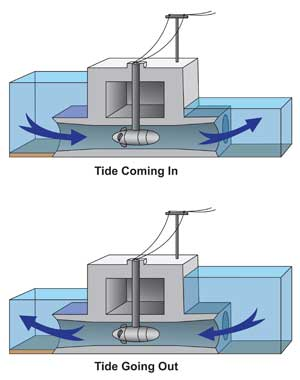
\includegraphics[height=0.35\textwidth]{res/cap 3/Tidal-power-300}
    \caption{Schema esemplificativo di impianto a bacino}
\end{figure}\noindent
\vfill
\newpage
\paragraph{Impatto ambientale}\mbox{}\\
L'impatto ambientale va considerato sia nella fase di costruzione che nella fase di operatività dell'impianto: nella prima, è richiesta la realizzazione di dighe o sbarramenti per creare bacini artificiali per l'accumulo di acqua.
Ciò può portare a una variazione dell'habitat marino e dell'ecosistema locale. Inoltre, la costruzione dell'impianto richiede la movimentazione di grandi quantità di terra e la costruzione di strutture portanti, che possono danneggiare o distruggere habitat naturali importanti.\\
Durante la fase di esercizio, invece, le centrali possono influenzare la salinità e la temperatura dell'acqua in mare aperto e nelle zone costiere. L'acqua che viene rilasciata dal bacino artificiale può avere una temperatura ed una salinità diversa rispetto all'acqua circostante, ciò può influire sulla flora e fauna marina locale. In aggiunta, le turbine e le altre componenti meccaniche dell'impianto possono rappresentare un rischio per la fauna marina, come i mammiferi marini o i pesci migratori, che possono rimanere intrappolati o essere feriti.\\
\section{Impianti idroelettrici}
In questa sezione sono descritti tutti quegli impianti che sfruttano l'energia dell'acqua in un punto nella fase del ciclo dalla sorgente al mare.\\
In un impianto si possono identificare due bacini: uno di monte, uno di valle ed una condotta che li collega che può essere a pelo libero od in pressione. In un punto intermedio tra i due bacini sarà collocata la centrale idroelettrica nella quale avverrà la conversione dell'energia cinetica dell'acqua in energia elettrica.\\
Questa tipologia di impianti sfrutta quindi l'energia potenziale del bacino di monte la quale, perdendo quota, acquisirà energia cinetica che andrà poi elaborata all'interno della centrale dalla turbina.\\
\begin{figure}[H]
    \centering
    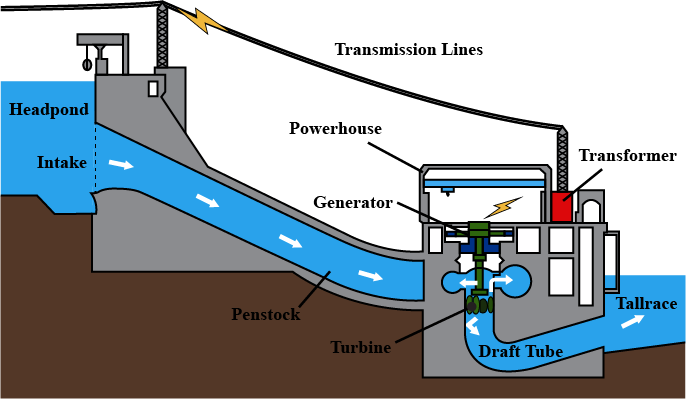
\includegraphics[height=0.4\textwidth]{res/cap 3/hpp diagram}
    \caption{Schema di una centrale idroelettrica}
\end{figure}\noindent
Sono presenti tre tipologie principali di turbine che andranno scelte in base al contesto specifico:
\begin{itemize}
    \item Pelton
    \item Francis
    \item Kaplan
\end{itemize}
\vfill
\newpage
\begin{figure}[H]
    \centering
    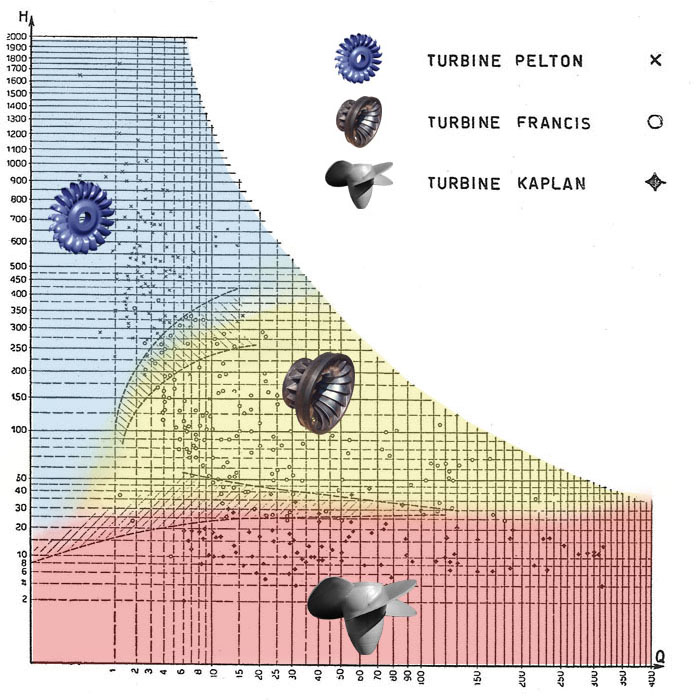
\includegraphics[height=0.4\textwidth]{res/cap 3/1_Campi-applicazione}
    \caption{Schema illustrativo dei campi di applicazione delle tre tipologie}
\end{figure}\noindent
Come è possibile vedere, le turbine Pelton sono in grado di elaborare una piccola portata ma un grande salto; Le Francis si posizionano invece con caratteristiche intermedie tra le due. Le Kaplan, invece, sono in grado di elaborare grandi portate ma con un salto contenuto.\\
Prima di illustrare singolarmente le caratteristiche delle tre tipologie è importante descrivere il funzionamento del Tubo aspiratore diffusore(TAD),un componente di fondamentale importanza per le ultime due in quando permette un grande recupero di energia che altrimenti andrebbe dispersa.
\subsection{Tubo aspiratore diffusore}
Il TAD è un condotto che ha il compito di collegare lo scarico della turbina con il bacino di valle:
\begin{figure}[H]
    \centering
    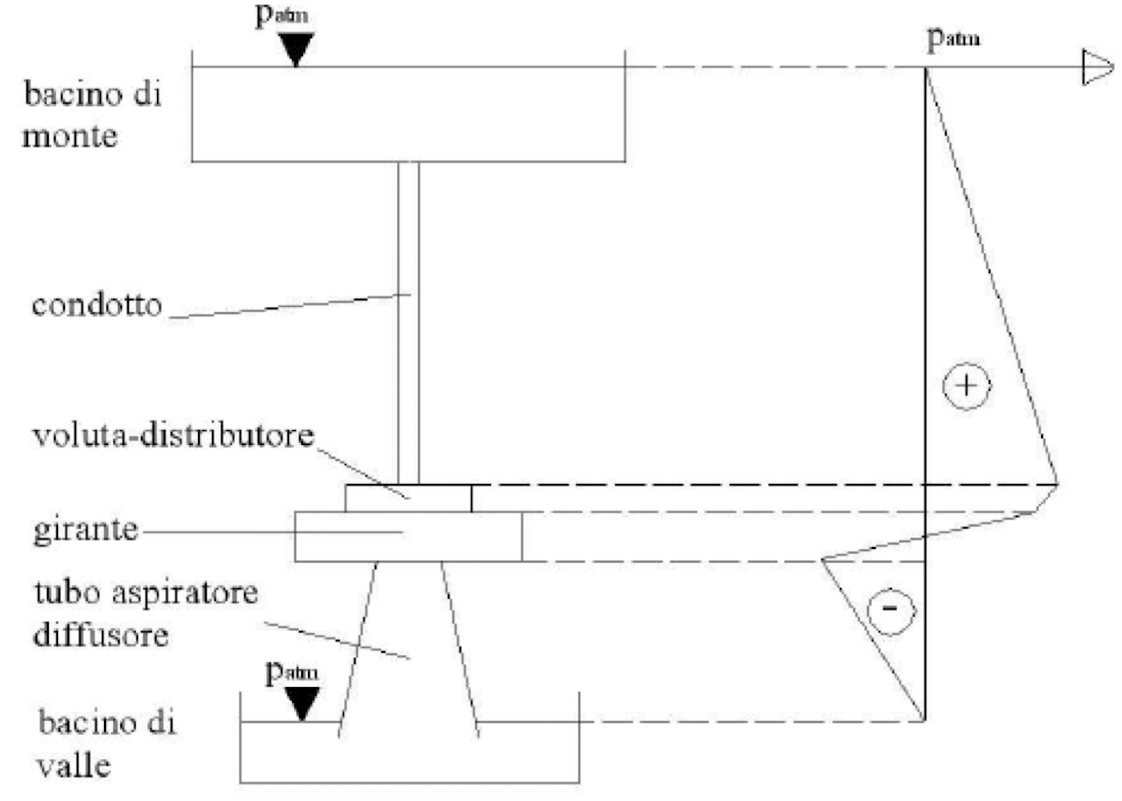
\includegraphics[height=0.4\textwidth]{res/cap 3/francis con TAD}
    \caption{Importanta del TAD}
\end{figure}\noindent
Questo componente infatti permette il recupero di parte dell'energia cinetica e del salto a valle ed di fondamentale importanza nelle turbine Francis e Kaplan.\\
Per spiegarne il funzionamento vengono illustrati tre scenari che si possono configurare a valle della turbina:
\begin{enumerate}
    \item Scarico a pressione atmosferica senza condotta
    \item Scarico con condotta a sezione costante
    \item Scarico con condotta a sezione variabile(TAD)
\end{enumerate}
Nel primo caso il salto a valle e l'energia cinetica vengono persi, installando un tubo a sezione costante si riesce a recuperare il salto a valle ma non l'energia cinetica mentre nel terzo caso è possibile recuperare entrambe.
Applicando il teorema di Bernoulli:
\begin{center}
    {\large$p_1+\frac{1}{2}\rho v_1^2 + \rho g h_1 = p_2+\frac{1}{2}\rho v_2^2 + \rho g h_2$}
\end{center}
La densità del fluido rimane costante, mentre {\large$p_2$} corrisponde alla pressione atmosferica, possiamo poi indicare la velocità come rapporto tra la portata e la sezione.
\begin{center}
    {\large$p_1+\frac{1}{2}\rho \frac{Q}{s_1}^2 + \rho g h_1 = p_{atm}+\frac{1}{2}\rho \frac{Q}{s_2}^2 + \rho g h_2$}
\end{center}
Nel caso di un tubo a sezione costante il secondo termine da entrambe le parti può essere semplificato in quando non varia. Trovandosi con la seguente relazione:
\begin{center}
    {\large$p_1 + \rho g h_1 = p_{atm}+ \rho g h_2$}
\end{center}
La pressione in uscita dalla turbina risulta quindi:
\begin{center}
    {\large$p_1 = p_{atm} + \rho g (h_2 - h_1)$}
\end{center}
Essendo la quota di scarico inferiore alla quota di aspirazione ci si trova ad avere una pressione {\large$p_1<p_{atm}$}, elaborando quindi parte dell'energia che sarebbe altrimenti andata persa.\\
Aggiungendo invece una sezione variabile ci si trova a non avere il secondo elemento costante:
\begin{center}
    {\large$p_1 = p_{atm} + \frac{1}{2}\rho Q^2 (\frac{1}{s_2^2} - \frac{1}{s_1^2}) + \rho g (h_2 - h_1)$}
\end{center}
In questo caso anche il secondo fattore sarà negativo in quanto il TAD ha una sezione in ingresso più piccola di quella in uscita, si ottiene perciò un'ulteriore recupero di salto piezometrico.\\
Le caratteristiche geometriche di questo condotto vanno attentamente studiate in quando un'errata progettazione potrebbe portare ad un fenomeno chiamato cavitazione.
Il fluido, allo scarico della turbina, trovandosi a bassissima pressione subisce un cambiamento di stato trasformandosi in vapore e subendo un grande aumento di volume.
Il vapore avendo un volume maggiore dell'acqua genera un aumento della velocità del fluido, ma una volta tornato ad una pressione che lo riporta in uno stato liquido può generare onde di pressione che rischiano di danneggiare i componenti meccanici.
\vfill
\newpage
\subsection{Pelton}
Questa tipologia, come precedentemente spiegato, è in grado di elaborare un grande salto(400-1800 m) ma portate medio piccole(1-10$\frac{m^3}{s}$), ottenendo quindi un range di potenza indicativo di 100-300MW.\\
E' una turbina ad azione($\varepsilon=0$), ciò indica che il salto piezometrico che il fluido mette a disposizione è elaborato solamente dall'organo distributore.\\
\begin{figure}[H]
    \centering
    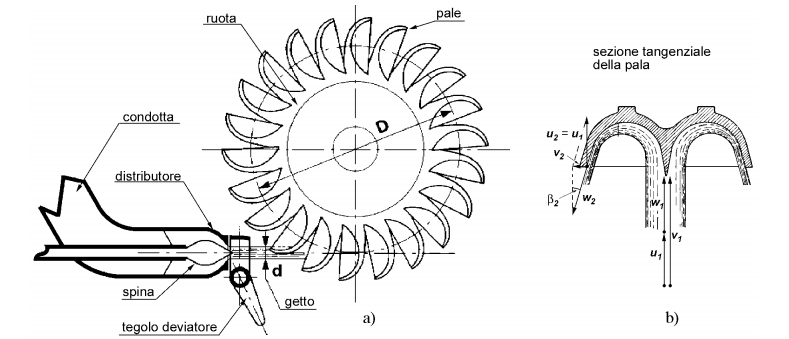
\includegraphics[height=0.4\textwidth]{res/cap 3/pelton}
    \caption{Schema di comprendente gli elementi principali di una turbina Pelton}
\end{figure}\noindent
In questa tipologia di turbine, dovendo operare con salti notevoli, l'acqua arriva all'interno di una condotta forzata. Il flusso poi viene deviato e raggiunge il/gli ugello/i la cui numerosità è definita dalla portata dell'acqua.
Una volta raggiunti gli ugelli la \enquote{spina doble} permette di convertire la pressione del fluido in energia cinetica indirizzando un getto direttamente sui cucchiai della girante la quale ruotando trasmette energia meccanica all'alternatore.\\
Il rendimento massimo ottenibile in questo tipo di turbina, nel caso ideale, si ottiene quando ci si trova ad avere un rapporto $\frac{u}{c_1}=0.5$ dove $c_1$ rappresenta la velocità dell'acqua e $u$ rappresenta la velocità periferica della ruota.
Noti i parametri di portata e caduta è opportuno progettare la macchina perché rispetti quel rapporto:\\
\begin{enumerate}
    \item Conoscendo la portata Q posso definire diversi parametri:\\
        \begin{center}
            {\large$Q=\frac{\pi}{4}\cdot d^2 \cdot c_1 \cdot i$}
        \end{center}
        Con d il diametro del getto, {\large$c_1$} la velocità in uscita del getto ed i il numero degli iniettori
    \item Ricavati d e {\large$c_1$} voglio che la macchina lavori ad {\large$\eta$} massimo che si ottime con un rapporto \large{$\frac{u}{c_1}=0.5$} noto \large{$c_1$} posso ricavare u e tramite la legge {\large$u=\omega r$} posso ricavare il raggio della girante
\end{enumerate}
Per il progetto della geometria della turbina sono invece ben definire le geometrie degli angoli delle pale.
\vfill
\newpage
\subsection{Francis}
Questa tipologia di turbina è quella tra le tre più polivalenti, è in grado infatti di elaborare portate in un range molto ampio(4-150{\large$\frac{m^3}{s}$}) ma anche salti notevoli(40-400m). Queste caratteristiche le permettono un ampio spettro di applicazione con potenze che, anche in questo caso, oscillano tra i 100 ed i 300MW.\\
A differenza della precedente la Francis è una turbina a reazione($\varepsilon>0$) ciò significa che in questo caso anche la girante contribuisce ad elaborare il salto piezometrico.
\begin{figure}[H]
    \centering
    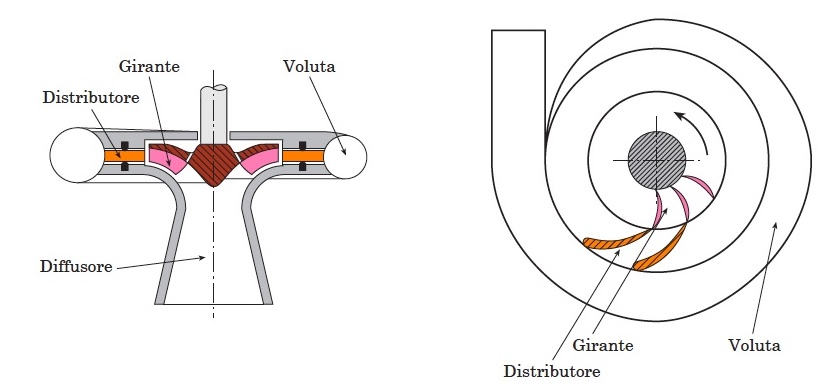
\includegraphics[height=0.4\textwidth]{res/cap 3/francis}
    \caption{Schema di una turbina Francis}
\end{figure}\noindent
In questo caso l'acqua inizia a scorrere all'interno della voluta la quale ha appositamente una sezione variabile in modo da poter mantenere costante la velocità del fluido al suo interno.
L'acqua a questo punto attraversa il distributore il quale ha una serie di pale orientabili le quali hanno lo scopo di elaborare la prima parte del salto piezometrico convertendo parte della pressione del fluido in velocità, è fondamentale che le pale siano orientabili in quanto permettono la regolazione della macchina.\\
La girante ha la caratteristica che ricevere il fluido radialmente e di scaricarlo assialmente convertendo l'energia cinetica dell'acqua in energia meccanica.
Di fondamentale importanza allo scarico è l'inserimento di un TAD per permettere una miglior efficienza.\\
Per quanto riguarda la fase progettuale ci si basa sulle caratteristiche di turbine già esistenti e funzionanti: si conosce la portata(Q), il salto piezometrico(H) ed il numero di giri a cui la macchina deve operare(n). Da esse tramite diagrammi specifici si possono ricavare tutti i parametri dimensionali.
\vfill
\newpage
\subsection{Ad elica o Kaplan}
Questa tipologia di turbina permette di elaborare portate elevate(>100{\large$\frac{m^3}{s}$}) però con salti contenuti(<90m), queste caratteristiche la collocano in ambito d'utilizzo molto specifico raggiungendo però solitamente potenze inferiori a quelle delle altre turbine(<200MW).\\
Anche in questo caso ci troviamo davanti ad una turbina a reazione con un Kq solitamente superiore alle Francis.
La differenza sostanziale tra le turbine ad elica e le Kaplan sta nel fatto che le seconde possono far variare il calettamento delle pale rotoriche oltre che quello delle pale del diffusore, permettendo di raggiungere il massimo grado di efficienza in condizioni diverse.
\begin{figure}[H]
    \centering
    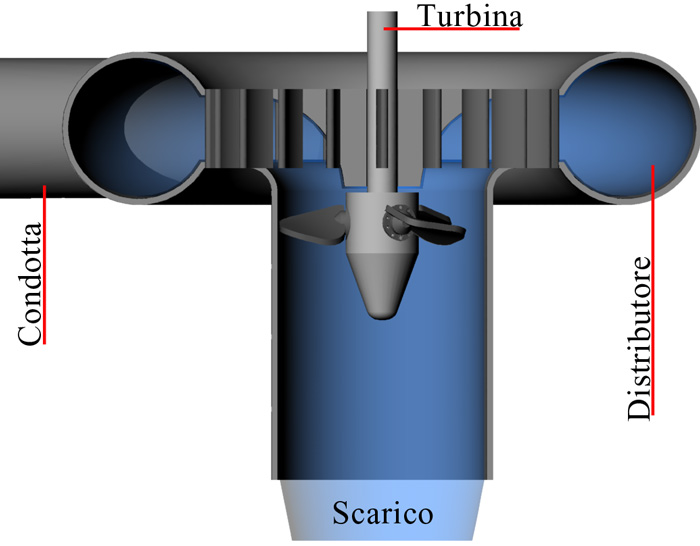
\includegraphics[height=0.4\textwidth]{res/cap 3/kaplan}
    \caption{Schema di una turbina Kaplan}
\end{figure}\noindent
Anche in questo caso a livello progettuale si parte dal fatto che si conoscano i principali parametri quali portata, salto e numero di giri della turbina(Q,H,n) e tramite una serie di tabelle caratteristiche si calcolano i parametri dimensionali della macchina.